% Establece la clase del documento y las especificaciones de la misma.
\documentclass[28pt, a4paper]{report}

%%%%%%%%%%%%%%%%%%%%%%%%%%%%%%%%%%%%%%%%%%%%%%%%%%%%%%%%%%%%%%%%%%%%%%%%%%%%%%%%%%%%%%%%%%%%%%%%%%%%%%%%%%%%%%%%%%%%%%%%%%%%%%%%%

% Establece el tamaño de los bordes de la página.
\usepackage[top=2cm, bottom=2cm, left=2cm, right=2cm]{geometry}
% Permite el uso de hipervínculos en el documento.
\usepackage{hyperref}
% Establece que el documento va a ser escrito en español (méxico).
\usepackage[spanish]{babel}
% Permite el control sobre la Tabla de Contenidos, Figuras, etc.
\usepackage{tocloft}
% Fuente y Tipografía.
\usepackage[sfdefault,lf]{carlito}
% Asegura el uso de "Unicode Transformation Format 8-bit" para asegurar el uso de carácteres modernos.
\usepackage[utf8]{inputenc}
% Permite el uso de espaciado entre carácteres, líneas, etc.
\usepackage{setspace}
% Permite el uso de ítems con diferente forma.
\usepackage{enumitem}
% Permite el uso de textos alineados al centro, izquierda o derecha de la página.
\usepackage{ragged2e}
% Permite el uso de títulos, encabezados y pies de página.
\usepackage{titlesec}
% Permite el uso de un formato encabezados y pies de página de una forma más amigable al lector.
\usepackage{fancyhdr}
% Permite el uso de más colores.
\usepackage{xcolor}
% Permite el uso de Apéndices.
\usepackage{appendix}

%%%%%%%%%%%%%%%%%%%%%%%%%%%%%%%%%%%%%%%%%%%%%%%%%%%%%%%%%%%%%%%%%%%%%%%%%%%%%%%%%%%%%%%%%%%%%%%%%%%%%%%%%%%%%%%%%%%%%%%%%%%%%%%%%

% Permite la inserción de imágenes al archivo.
\usepackage{graphicx}
% Permite el uso de imágenes y figuras rotadas
\usepackage{rotating}
% Permite cambiar el tamaño de las imágenes.
\usepackage[export]{adjustbox}
% Permite el uso de hojas apaisadas y verticales.
\usepackage{pdflscape}
% Permite el uso de múltiples imágenes dentro de una figura.
\usepackage{subcaption}
% Permite la definición de objetos flotantes como tablas e imágenes.
\usepackage{float}
% Expande las capacidades de las tablas.
\usepackage{array}
% Expande las capacidades de las tablas.
\usepackage{tabularx}
% Expande las capacidades de las tablas.
\usepackage{tabularray}
%%%%%%%%%%%%%%%%%%%%%%%%%%%%%%%%%%%%%%%%%%%%%%%%%%%%%%%%%%%%%%%%%%%%%%%%%%%%%%%%%%%%%%%%%%%%%%%%%%%%%%%%%%%%%%%%%%%%%%%%%%%%%%%%%

% Permite el uso de ecuaciones y distintos formatos de las mismas.
\usepackage{amsmath}
% Permite el uso de fracciones de una forma que ocupe menos espacio y sea más legible.
\usepackage{graphicx, nicefrac}
% Permite el uso de cancelaciones en una ecuación.
\usepackage{cancel}
% Permite poner código como si fuera una términal de código.
\usepackage{listings}

%%%%%%%%%%%%%%%%%%%%%%%%%%%%%%%%%%%%%%%%%%%%%%%%%%%%%%%%%%%%%%%%%%%%%%%%%%%%%%%%%%%%%%%%%%%%%%%%%%%%%%%%%%%%%%%%%%%%%%%%%%%%%%%%%

% Establece que la carpeta a usar para almacenar las imágenes es "Imagenes".
\graphicspath{Imagenes/}

%%%%%%%%%%%%%%%%%%%%%%%%%%%%%%%%%%%%%%%%%%%%%%%%%%%%%%%%%%%%%%%%%%%%%%%%%%%%%%%%%%%%%%%%%%%%%%%%%%%%%%%%%%%%%%%%%%%%%%%%%%%%%%%%%

% Establece la separación entre líneas.
\setlength{\lineskip}{3.5pt}
% Establece la mínima separación entre líneas.
\setlength{\lineskiplimit}{2pt}
% Establece la sangría.
\setlength{\parindent}{20pt}
% Establece la separación entre parráfos.
\setlength{\baselineskip}{12pt}

%%%%%%%%%%%%%%%%%%%%%%%%%%%%%%%%%%%%%%%%%%%%%%%%%%%%%%%%%%%%%%%%%%%%%%%%%%%%%%%%%%%%%%%%%%%%%%%%%%%%%%%%%%%%%%%%%%%%%%%%%%%%%%%%%

\titleclass{\subsubsubsection}{straight}[\subsection]

\newcounter{subsubsubsection}[subsubsection]
\renewcommand\thesubsubsubsection{\thesubsubsection.\arabic{subsubsubsection}}
\renewcommand\theparagraph{\thesubsubsubsection.\arabic{paragraph}}

\titleformat{\subsubsubsection}
  {\normalfont\normalsize\bfseries}{\thesubsubsubsection}{1em}{}
\titlespacing*{\subsubsubsection}
{0pt}{3.25ex plus 1ex minus .2ex}{1.5ex plus .2ex}

\makeatletter
\renewcommand\paragraph{\@startsection{paragraph}{5}{\z@}%
  {3.25ex \@plus1ex \@minus.2ex}%
  {-1em}%
  {\normalfont\normalsize\bfseries}}
\renewcommand\subparagraph{\@startsection{subparagraph}{6}{\parindent}%
  {3.25ex \@plus1ex \@minus .2ex}%
  {-1em}%
  {\normalfont\normalsize\bfseries}}
\def\toclevel@subsubsubsection{4}
\def\toclevel@paragraph{5}
\def\toclevel@paragraph{6}
\def\l@subsubsubsection{\@dottedtocline{4}{7em}{4em}}
\def\l@paragraph{\@dottedtocline{5}{10em}{5em}}
\def\l@subparagraph{\@dottedtocline{6}{14em}{6em}}
\makeatother

\setcounter{secnumdepth}{4}
\setcounter{tocdepth}{4}

%%%%%%%%%%%%%%%%%%%%%%%%%%%%%%%%%%%%%%%%%%%%%%%%%%%%%%%%%%%%%%%%%%%%%%%%%%%%%%%%%%%%%%%%%%%%%%%%%%%%%%%%%%%%%%%%%%%%%%%%%%%%%%%%%

% Establece las condiciones para los hipervínculos.
\hypersetup{colorlinks=true,linkcolor=medium_violet,filecolor=dark_violet,urlcolor=light_violet,pdftitle={Carpeta Técnica GraviCap},pdfpagemode=FullScreen,}

%%%%%%%%%%%%%%%%%%%%%%%%%%%%%%%%%%%%%%%%%%%%%%%%%%%%%%%%%%%%%%%%%%%%%%%%%%%%%%%%%%%%%%%%%%%%%%%%%%%%%%%%%%%%%%%%%%%%%%%%%%%%%%%%%

% Establece el estilo de la página para permitir el uso de encabezados y pies de página.
\pagestyle{fancy}
% Establece el uso de encabezados y pies de página.
\fancyhf{}
% Establece el contenido de la parte izquierda del encabezado.
\lhead{\footnotesize \textcolor{dark_violet}{\textbf{GraviCap}} - \the\year{}}
% Establece el contenido de la parte central del encabezado.
\chead{
\includegraphics[width=1cm]{Imagenes/Preface/IMPA.png}}
% Establece el contenido de la parte de derecha del encabezado.
\rhead{\footnotesize E.E.S.T N°7 IMPA "T.R.Q."}
% Establece el contenido de la parte central del pie de página.
\cfoot{\large \thepage}

%%%%%%%%%%%%%%%%%%%%%%%%%%%%%%%%%%%%%%%%%%%%%%%%%%%%%%%%%%%%%%%%%%%%%%%%%%%%%%%%%%%%%%%%%%%%%%%%%%%%%%%%%%%%%%%%%%%%%%%%%%%%%%%%%%

% Establece que dentro de la tipografía "Carlito" se use la variante "OsF".
\renewcommand*\oldstylenums[1]{\carlitoOsF #1}
% Establece el tamaño del pie de página.
\renewcommand{\footrulewidth}{0.4pt}
% Establece que en la tabla de contenidos se use una línea de puntos para marcar el número de página.
\renewcommand{\cftsecleader}{\cftdotfill{\cftdotsep}}
% Establece un color con los valores 102, 19, 154 en RGB.
\providecolor{medium_violet}{RGB}{102,19,154}
% Establece un color con los valores 169, 68, 238 en RGB.
\providecolor{light_violet}{RGB}{169,68,238}
% Establece un color con los valores 81, 9, 129 en RGB.
\providecolor{dark_violet}{RGB}{81,9,129}

\definecolor{codegreen}{rgb}{0,0.6,0}
\definecolor{codegray}{rgb}{0.5,0.5,0.5}
\definecolor{codepurple}{rgb}{0.58,0,0.82}
\definecolor{backcolour}{rgb}{0.95,0.95,0.92}

%%%%%%%%%%%%%%%%%%%%%%%%%%%%%%%%%%%%%%%%%%%%%%%%%%%%%%%%%%%%%%%%%%%%%%%%%%%%%%%%%%%%%%%%%%%%%%%%%%%%%%%%%%%%%%%%%%%%%%%%%%%%%%%%%

\lstdefinestyle{mystyle}{
    backgroundcolor=\color{backcolour},   
    commentstyle=\color{codegreen},
    keywordstyle=\color{magenta},
    numberstyle=\tiny\color{codegray},
    stringstyle=\color{codepurple},
    basicstyle=\ttfamily\footnotesize,
    breakatwhitespace=false,         
    breaklines=true,                 
    captionpos=b,                    
    keepspaces=true,                 
    numbers=left,                    
    numbersep=5pt,                  
    showspaces=false,                
    showstringspaces=false,
    showtabs=false,                  
    tabsize=2
}

\lstset{style=mystyle}

%%%%%%%%%%%%%%%%%%%%%%%%%%%%%%%%%%%%%%%%%%%%%%%%%%%%%%%%%%%%%%%%%%%%%%%%%%%%%%%%%%%%%%%%%%%%%%%%%%%%%%%%%%%%%%%%%%%%%%%%%%%%%%%%%

\begin{document}
\begin{titlepage}

        \begin{center}      
            \begin{figure} [!ht]
                \centering
                
\includegraphics [width=9cm]{Imagenes/Preface/Logo-Nombre.png}
                \label{Logo-Nombre}
            \end{figure}
            
                \vspace{0.5cm}
                {\LARGE\textbf{{\textcolor{dark_violet}{\textbf{\textit{Una forma de elevar tu energía}}}}}}\par
                \vspace{0.5cm}
            {\Huge\textbf{Manual de Usuario}}\par
                \vspace{1cm}
            {\LARGE\textbf{7mo 1ra Comisión A}}\par
                \vspace{0.2cm}
            {\LARGE\textbf{Año \the\year}}\par
                \vspace{1cm}
            {\Large\textbf{{Alvarez Mollo, Fausto}}}\par
            {\Large\textbf{{Bianqui Kronemberger, Mariano Joaquín}}}\par
            {\Large\textbf{{Calleja, Tomás Joaquín}}}\par
            {\Large\textbf{{Donatti, Augusto}}}\par
            {\Large\textbf{{Felizia, Tatiana Milena}}}\par
            {\Large\textbf{{Sofía, Gabriel Jerónimo Takashi}}}\par
                \vspace{1.5cm}
            \begin{figure} [!ht]
                \centering
                
\includegraphics [width=7cm]{Imagenes/Preface/IMPA.png}
                \label{IMPA}
            \end{figure}
        \end{center}
        
    \end{titlepage}
    
%%%%%%%%%%%%%%%%%%%%%%%%%%%%%%%%%%%%%%%%%%%%%%%%%%%%%%%%%%%%%%%%%%%%%%%%%%%%%%%%%%%%%%%%%%%%%%%%%%%%%%%%%%%%%%%%%%%%%%%%%%%%%%%%%%%%%%%%%%%%%%%
    \tableofcontents
    \newpage
%%%%%%%%%%%%%%%%%%%%%%%%%%%%%%%%%%%%%%%%%%%%%%%%%%%%%%%%%%%%%%%%%%%%%%%%%%%%%%%%%%%%%%%%%%%%%%%%%%%%%%%%%%%%%%%%%%%%%%%%%%%%%%%%%%%%%%%%%%%%%%%

\chapter{Introducción}
    \section{¿Qué es \textcolor{dark_violet}{GraviCap}?}
        \textcolor{dark_violet}{GraviCap} (Gravity Capacitor) es una batería de almacenamiento gravitatorio. Su finalidad es igual a una batería convencional, pero con un funcionamiento de generación de energía totalmente distinto e innovador.\par

    \section{Funcionamiento Principal}
        Esta batería está conformada por una estructura, la cual eleva un peso por medio de un motor, un sistema de poleas y un cable de acero, almacenando energía potencial gravitatoria en el peso. Cuando se necesita energía en el dispositivo que queramos cargar, el motor hará descender la masa de manera controlada, generando energía eléctrica gracias al movimiento del motor al ser movido por el cable.\par

    \section{Objetivos}
        Teniendo en cuenta como fenómeno mundial, la contaminación por baterías convencionales, ya sea de litio, de autos o de celulares, surge nuestro objetivo principal, darle al mundo una nueva alternativa de almacenamiento de energía por medio de nuestro producto, trayendo a nuestro país una nueva forma de batería, siendo ideal para usarla con energías renovables, no contaminantes y sustentables. Finalmente presentando al mundo una forma sustentable y no contaminante de almacenar energía.\par
        
    \section{Beneficios}
        \begin{itemize}
            \item Nuestra batería, al tener como factor principal aprovechar la energía potencial gravitatoria para la generación de energía eléctrica, es completamente sustentable y no contaminante para el medio ambiente.\par
            \item Esta forma de generación de energía es poco vista e implementada dentro del mundo y de las primeras utilizadas en Argentina. Siendo así, una nueva forma vanguardista de batería dentro de nuestro país.
            \item Puede aprovecharse lugares o infraestructuras en desuso para la instalación de la batería. Por ejemplo, minas abandonadas, contando con una gran profundidad para el recorrido del peso. También, puede aprovecharse una torre de control de un aeródromo o aeropuerto, contando con una gran altura para un eficiente funcionamiento y recorrido del peso. 
            \item El sistema de almacenamiento de energía sobrante de las fuentes utilizadas, garantiza para el usuario una estabilidad de energía en la batería en los momentos de pico o baja consumo aprovechando al máximo lo que genera.
            \item Gracias al sistema mecánico de \textcolor{dark_violet}{GraviCap} se producen menos desgastes en la estructura en la carga y descarga de energía, así proporcionando una vida útil más larga que una batería convencional y, por ende, menos coste de mantenimiento. 
            \item Permite monitorear el funcionamiento del sistema \textcolor{dark_violet}{GraviCap} por medio de una aplicación móvil.
        
        \end{itemize}
\chapter{Aplicación}

    \section{Función de la aplicación}
        La aplicación móvil tiene como objetivo mostrarle al usuario los distintos tipos de valores de la batería en tiempo real. Esto lo hará por medio de pantallas destinadas a los valores e interacciones que necesite el usuario, contando con gráficos interactivos. Los datos mostrados en la aplicación son subidos desde una base de datos. Contando también con una sección para contactarnos, por medio de nuestras redes sociales y página web.\par
        Con esta aplicación, el usuario podrá saber, en todo momento, los valores que necesite de la batería, como por ejemplo, la entrega que tiene la batería hacia el dispositivo que esté alimentando o, para un perfil más técnico, valores del panel solar y gráficos para más detalles sobre la misma.\par

    \section{Desarrollo del mockup de la aplicación}
    
        \subsection{Mockup}
            	Para poder desarrollar la aplicación, se necesita tener un Mockup. Su función es proveer al desarrollador el prototipo de funcionamiento, planteado de forma ilustrativa, el cual, da un primer vistazo estético, funcional e informativo de cómo será la misma. \par
                Esto conlleva plantear el diseño, e información que contendrá la aplicación , para que, posteriormente, el desarrollo final de la aplicación, se base en el Mockup, siendo de esta forma, más cómodo y práctico poder desarrollarla.\par
                La página que se designó para realizar el Mockup, fue “\href{https://marvelapp.com}{Marvel}”.\par
                Dentro de este, pueden haber varios cambios según vaya avanzando y se necesite, ya que, al fin y al cabo, es a modo ilustrativo para después poder desarrollar la aplicación final.\par
                
                \begin{figure}[H]
                    \centering
                    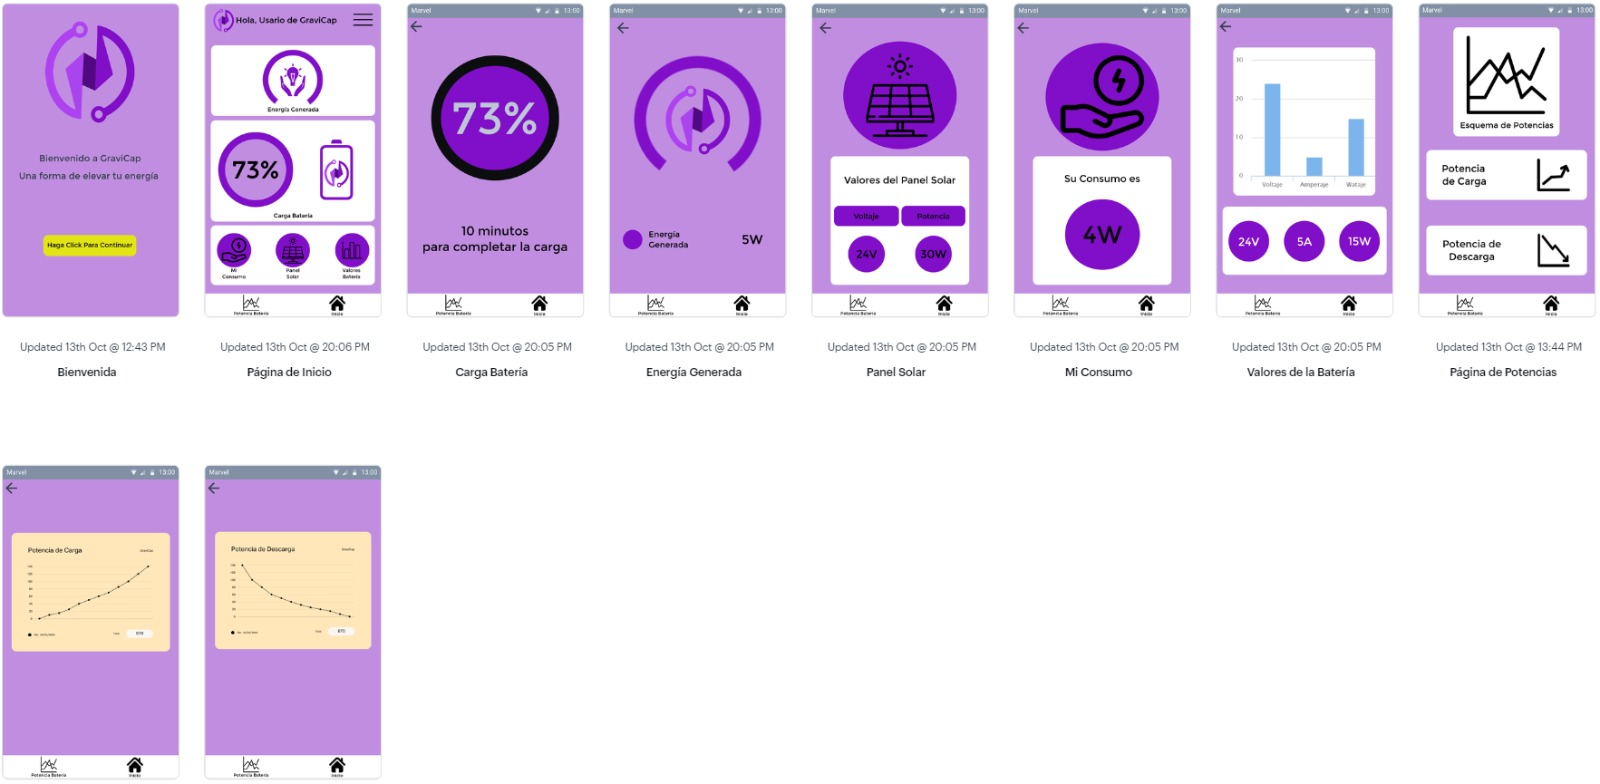
\includegraphics[width=0.8\linewidth]{Imagenes/Aplicación/Mockup.jpg}
                    \caption{Mockup de la aplicación.}
                    \label{fig:a14}
                \end{figure}
                
            \subsection{UI/UX}
                La \textbf{UX} (Experiencia de Usuario) es la experiencia integral y el conjunto de interacciones que tienen los usuarios con la misma.\par
                En cuanto a la \textbf{UI} (Interfaz de Usuario) consiste en toda la arquitectura de información, patrones y diferentes elementos visuales que nos permitan explorar la funcionalidad de la aplicación de forma eficaz y gratificante.\par
                Con esto, el usuario podrá tener una interacción “amigable” con la aplicación, siendo más cómodo y práctico moverse dentro de la misma para ver lo que necesite.\par
                La diferencia entre estos, es que la UX se centra en la manera en que el usuario interactúa con el producto de manera eficaz y, por otro lado, la UI busca ofrecer una experiencia estética satisfactoria.\par

            \subsection{User Journey}
                Para el desarrollo de la aplicación se planteó utilizar como metodología, una “jornada de usuario”. Esta metodología, plantea un mapa de recorrido del usuario en nuestra aplicación, representando así, su experiencia visual e interactiva con la misma. Pudiendo así, plantear el desarrollo del Mockup enfocándonos en el proceso que realizaría nuestro usuario dentro de la aplicación y su perspectiva.\par
                El proceso para esta metodología es buscar la empatía con el usuario, comprendiendo la relación y puntos de contacto que este tiene. Analizar sus acciones y procesos, para así, determinar lo que necesita. Con esto, se puede generar una mejor experiencia para el usuario y un proceso más eficiente.\par
                Facilita tanto el desarrollo de la aplicación como el proyecto en sí, generando una experiencia del usuario y requerimientos para el mismo. También se relaciona directamente con la UI/UX y facilita un mejor y cómodo planteamiento para las mismas.\par
                Esta herramienta o metodología, nos permite generar un usuario para así comprender y mejorar su experiencia dentro de la aplicación, así también, dándonos un mejor desarrollo dentro de nuestro proyecto.\par

                
        \section{Estructura de la Aplicación}
        
            \subsection{Editor de Código y Framework}
                Para el desarrollo de la aplicación, se utilizó el editor de código “Visual Studio Code”, en conjunto con “\href{https://ionicframework.com}{Ionic}" un framework de código abierto, proporcionandonos comodidad y amplias opciones de herramientas para el desarrollo, conteniendo varias opciones para la implementación en varios lenguajes.
                
            \subsection{Lenguajes Utilizados}
                Los lenguajes utilizados fueron HTML, CSS, JS y, como principal, React. Siendo este último, el lenguaje principal para el uso de las herramientas que nos provee Ionic.\par
                
            \subsection{Componentes}
        
                \subsubsection{WelcomePage.tsx}
                
                    Este componente es el primero que se ve al iniciar la aplicación, su función consta de darle una pequeña bienvenida al usuario, con nuestro logo y \textit{slogan}, explicando un poco sobre la batería, el proyecto, la funcionalidad de la aplicación y un botón que lo envía a la pantalla de inicio una vez que el usuario quiera.\par
    
                    \begin{figure} [H]
                        \centering
                        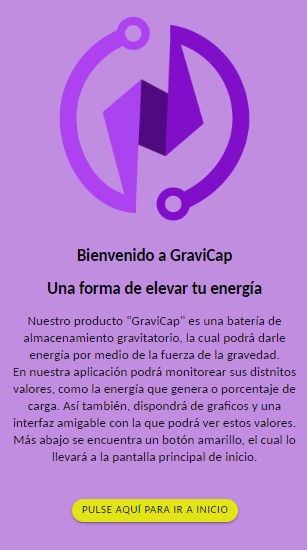
\includegraphics[width=0.25\linewidth]{Imagenes/Aplicación/Welcome.jpg}
                        \caption{Página de Bienvenida}
                        \label{fig:a1}
                    \end{figure}
                
                \subsubsection{StartPage.tsx}
                    Una vez vista la pantalla de bienvenida, el usuario es reenviado hacia la pantalla de inicio, la cual, es la pantalla principal de la aplicación, esta contiene los botones con links hacia las distintas pantallas de valores.En la parte inferiror izquierda de la página encontramos un botón amarillo de tamaño pequelo el cual le permite al usuario redirigirse hacia la pantalla de gráficos de potencia de la batería.\par
                    En el apartado de arriba a la derecha encontramos un botón de información, el cual contiene los links hacia nuestro contacto y diversas redes sociales.\par
                    
                    \begin{figure} [H]
                        \centering
                        \begin{subfigure}{0.4\textwidth}
                            \centering
                            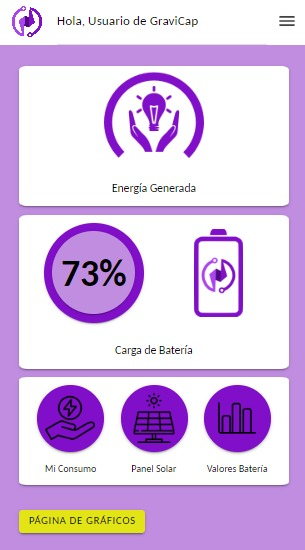
\includegraphics[width=0.7\textwidth]{Imagenes/Aplicación/Start.jpg}
                            \caption{Página de Inicio}
                            \label{fig:a2.1}
                        \end{subfigure}
                        \begin{subfigure}{0.4\textwidth}
                            \centering
                            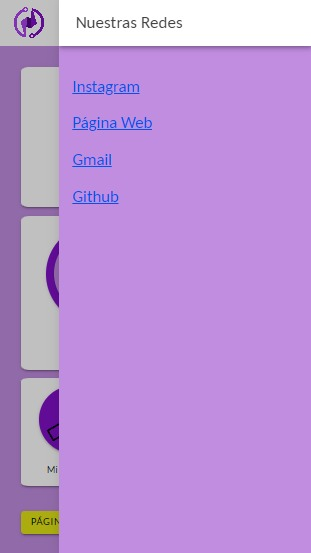
\includegraphics[width=0.7\textwidth]{Imagenes/Aplicación/Start_Menu.jpg}
                            \caption{Menú de Inicio}
                            \label{fig:a2.2}
                        \end{subfigure}
                        \hfill
                                
                        \caption{Ambas partes de la Página de Inicio}
                        \label{fig:a2}
                        \end{figure}
                
                \subsubsection{GeneratedEnergy.tsx}
                    Este componente contiene un valor importante y recurrente para el usuario, el cual es la energía generada por la batería. Este valor le provee al usuario el valor de cuánta potencia está entregando hacia su dispositivo.\par
                    En esta pantalla disponemos de un gráfico circular referenciando el valor de potencia de energía generada de la batería.\par
                    En la parte inferior encontramos el color referenciando el valor del gráfico con un texto plasmando el valor numérico textualmente con su unidad (Watt).\par
    
                    \begin{figure} [H]
                        \centering
                        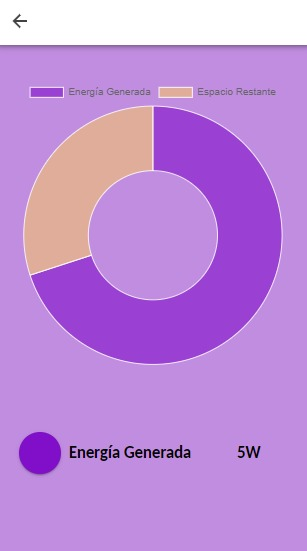
\includegraphics[width=0.25\linewidth]{Imagenes/Aplicación/Generated.jpg}
                        \caption{La cantidad de energía generada (Los valores son de referencia)}
                        \label{fig:a3}
                    \end{figure}
                
                \subsubsection{BatteryCharge.tsx}
                    Para el usuario, también es importante saber cuál es la carga de la batería, es decir, en este caso, si está en su punto más alto o más bajo. Este valor se basa en un porcentaje, el cual nos indica la posición del peso de la batería, que se traduce en un valor porcentual para el usuario. Por ejemplo, el 100\% de la batería, se da cuando el peso está en su punto más alto, ya habiendo almacenado la energía potencial gravitatoria. Por lo tanto, el 0\% referencia cuando el peso está en su punto más bajo, ya habiendo descargado toda la batería.\par
                    Este apartado también cuenta con el tiempo que falta para que la batería llegue a completar su carga.\par
    
                    \begin{figure} [H]
                        \centering
                        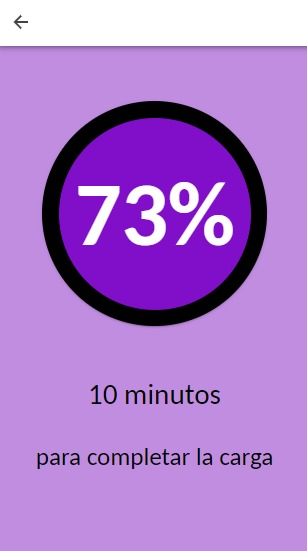
\includegraphics[width=0.25\linewidth]{Imagenes/Aplicación/Charge.jpg}
                        \caption{Carga de la batería (Los valores son de referencia)}
                        \label{fig:a4}
                    \end{figure}
                
                \subsubsection{MyConsumption.tsx}
                    El usuario también necesita saber el consumo de su dispositivo. Ese es el funcionamiento de este componente. Dándole el valor en unidad de potencia.\par
    
                    \begin{figure} [H]
                        \centering
                        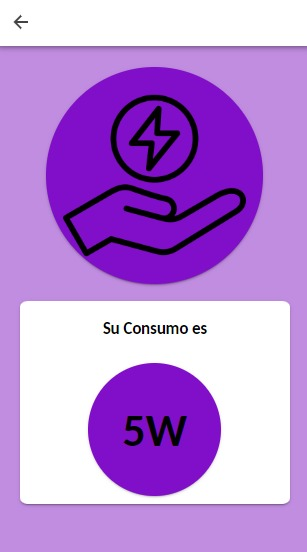
\includegraphics[width=0.25\linewidth]{Imagenes/Aplicación/Consumption.jpg}
                        \caption{El consumo del usuario (Los valores son de referencia)}
                        \label{fig:a5}
                    \end{figure}
                
                \subsubsection{SolarPanel.tsx}
                    Para saber los valores de entrega del panel solar, el usuario puede verlos dentro de la pantalla del panel solar.\par
                    Los valores que podemos ver son el voltaje que entrega y su potencia. Todo esto en tiempo real.\par
    
                    \begin{figure} [H]
                        \centering
                        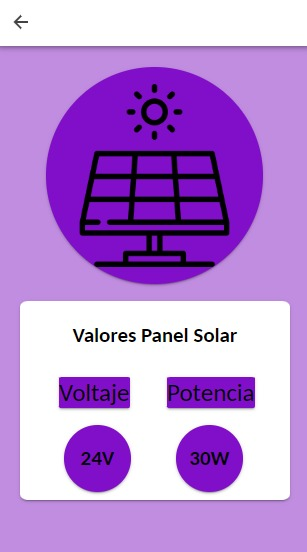
\includegraphics[width=0.25\linewidth]{Imagenes/Aplicación/Value_Energy.jpg}
                        \caption{Valor del panel solar utilizado (Los valores son de referencia)}
                        \label{fig:a6}
                    \end{figure}
                
                \subsubsection{BatteryValues.tsx}
                    Para registrar la batería y sus valores varios, en la pantalla de valores de batería el usuario podrá ver valores como Voltaje, Corriente y Potencia de la batería.\par
    
                    \begin{figure} [H]
                        \centering
                        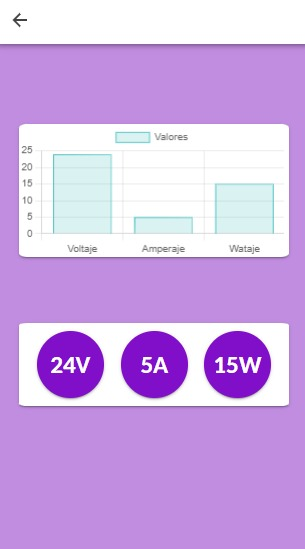
\includegraphics[width=0.25\linewidth]{Imagenes/Aplicación/Value_Battery.jpg}
                        \caption{Valor de la batería (Los valores son de referencia)}
                        \label{fig:a7}
                    \end{figure}

                \subsubsection{GraphicsPage.tsx}
                    En este apartado, el cual el usuario puede acceder desde el botón amarillo de la página de inicio, encontraremos dos botones los cuales contienen los gráficos de carga y descarga de la batería.\par
    
                    \begin{figure} [H]
                        \centering
                        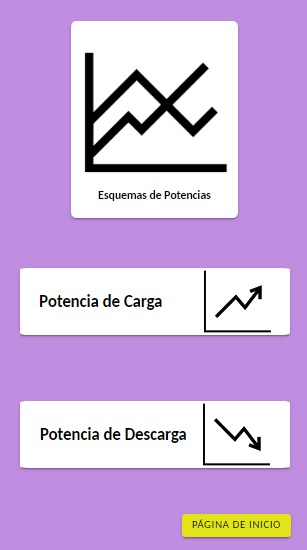
\includegraphics[width=0.25\linewidth]{Imagenes/Aplicación/Graphics_Page.jpg}
                        \caption{Página de Gráficos}
                        \label{fig:a8}
                    \end{figure}

                \subsubsection{ChargingPowerGraphics.tsx}
                    En esta pantalla encontramos un gráfico ascendente, el cual se basa en la potencia que entrega la batería en función del tiempo cuando el peso está en su momento de ascenso.\par
    
                    \begin{figure} [H]
                        \centering
                        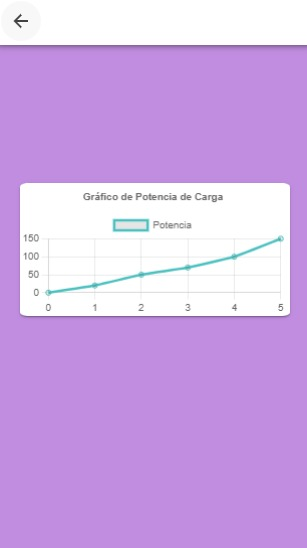
\includegraphics[width=0.25\linewidth]{Imagenes/Aplicación/Graphics_Charge.jpg}
                        \caption{Gráfico de Carga (Los valores son de referencia)}
                        \label{fig:a9}
                    \end{figure}

                \subsubsection{DischargePowerGraphics.tsx}
                    Esta pantalla actúa de igual forma que la anterior, encontraremos un gráfico descendente el cual se basa en la potencia que entrega la batería en función del tiempo.\par
                    Este funciona cuando la batería se encuentra en estado de descarga, es decir, cuando está descendiendo.\par
    
                    \begin{figure} [H]
                        \centering
                        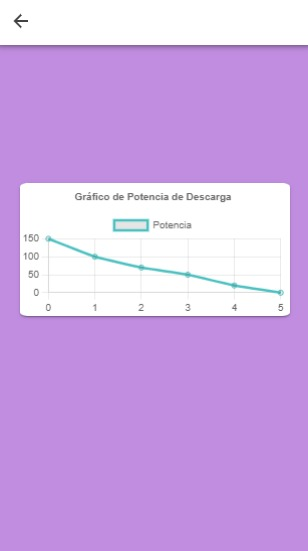
\includegraphics[width=0.25\linewidth]{Imagenes/Aplicación/Graphics_Discharge.jpg}
                        \caption{Gráfico de Descarga (Los valores son de referencia)}
                        \label{fig:a10}
                    \end{figure}

                \subsubsection{Buttons.tsx}
                    Este componente es un botón de tamaño pequeño amarillo ubicado en la parte inferior de la página de inicio, el cual está declarado con una ruta de navegación que permite conectar la página principal de inicio con la página de gráficos de potencia de la batería.\par 
                    También hay un botón del mismo estilo en la página de gráficos para poder volver hacia la pantalla principal de inicio si se necesita.\par 
                    Con esto, damos una forma eficiente de visualización de valores entre páginas por medio de estos botones.\par

                    \begin{figure}[H]
                        \centering
                        \begin{subfigure}{0.4\textwidth}
                            \centering
                            
\includegraphics[width=0.7\textwidth]{Imagenes/Aplicación/Start_Button.jpg}
                            \caption{Botón para volver a la Página de Inicio}
                            \label{fig:a15.1}
                        \end{subfigure}
                        \begin{subfigure}{0.4\textwidth}
                            \centering
                            
\includegraphics[width=0.7\textwidth]{Imagenes/Aplicación/Graphics_Button.jpg}
                            \caption{Botón para volver la página de Gráficos}
                            \label{fig:a15.2}
                        \end{subfigure}
                        \hfill
                                
                        \caption{Ambas partes de la Página de Inicio}
                        \label{fig:a20}
                        \end{figure}
                    
                \subsubsection{Tabs.tsx}
                    Este componente es la barra de botones que se encuentra en la parte de abajo, este contiene un botón que te redirecciona hacia la pantalla de inicio y otra que te redirecciona hacia la parte los gráficos de potencia. Dándole una mayor accesibilidad al usuario hacia las pantallas del Tab.\par

                \subsubsection{main.tsx}
                    El main es un componente el cual no es visible, dentro de la aplicación. Este se encarga de poder ejecutar las rutas declaradas dentro del archivo App.tsx.\par

                \subsubsection{App.tsx}
                    Este componente tampoco es visible, ya que se encarga de declarar las rutas dentro de la aplicación. Por ejemplo, puede realizar que al abrir la aplicación, redireccione al usuario hacia la pantalla de bienvenida.\par
                
        \section{Desarrollo}
            Para el desarrollo de la aplicación, se descargó \textbf{Ionic}, configurando su descarga para la utilización de herramientas y templates con el lenguaje de programación de \textbf{React}. Para poder programar y utilizar las herramientas descargadas se utilizó el editor de código de \textbf{Visual Studio Code}.\par 
            \subsection{Base de Datos}
                Teniendo como base de desarrollo el Mockup, facilita la programación de la misma. También cabe resaltar que mediante se desarrolla la aplicación en sí, el Mockup puede ir variando o la aplicación puede no ser completamente fiel estética y visualmente al mismo, quedando la aplicación final, diferente al Mockup, esto ya que se utiliza como una primera base.\par 
                Mediante el proceso se encuentran nuevas herramientas que se adapten mejor a las necesidades del momento, reescribiendo o modificando el Mockup según se requiera para una mejor versión de la aplicación.\par
                
            \subsection{Creación de Archivos}
                Se crearon los distintos archivos que funcionarán como componentes para la creación de las pantallas de la aplicación, desarrollando y programando así la estructura de cada uno, importando las carpetas y herramientas para cada archivo.\par

            \subsection{Herramientas de Ionic}
                Para el desarrollo de programación de los archivos se necesitó tener conocimientos dentro del lenguaje de HTML para poder programar su estructura y combinarse con el lenguaje principal React y las herramientas que provee, creando así, componentes .tsx como archivos principales para el desarrollo. En cuanto a las herramientas que nos provee Ionic, se investigó en el Framework sobre sus templates e información del uso de las herramientas más convenientes para el desarrollo de los archivos. Para poder estilizarlos según queramos, se necesitó también tener conocimientos en CSS. Para los gráficos, importados de carpetas, se necesitó tener conocimientos básicos en JavaScript.\par
                
                \subsubsection{IonApp}
                    Para la creación de los archivos, se necesita empezar con una constante o función, en la cual iremos desarrollando el código para la creación de las pantallas, así como declarar primeramente una herramienta IonApp la cual contendrá el código y los elementos de la aplicación de Ionic, solamente se declara uno en el archivo que queramos considerar como principal.\par
                
                \subsubsection{IonContent}
                    Otro componente importante para el desarrollo es declarar un IonContent el cual actúa de contenedor principal de los componentes de la aplicación, dando así, un área única para el contenido por fuera del Header.\par
                
                \subsubsection{IonHeader y IonMenu}
                    IonHeader componente que actúa de barra superior central, conteniendo componentes tales como iconos, botones y texto (vistos en el Header de la pantalla de Inicio). En este mismo también se declara el componente IonMenu, un botón de información lateral ubicado en la parte superior derecha de la pantalla de inicio, proporcionando los links hacia nuestras redes sociales, contacto y página web.\par
                
                \subsubsection{IonCard}
                    Un componente muy utilizado es el de IonCard visto en gran parte en la pantalla de inicio y utilizado en otros archivos. Actuando de contenedor de otros componentes y, a su vez, dándole una mejor estética, actuando, como dice su nombre, como una carta. Modificándose en cuanto a estilos y formas con CSS, pueden actuar de contenedores circulares, también vistos en los contenedores de "Mi Consumo", "Panel Solar" y "Valores de Batería" en la pantalla de inicio. También dándole un recuadro en las páginas de gráficos, y actuando como "botones" (declarados con el componente de NavLink los cuales, al clickearlos, nos redireccionan hacia otra pantalla.\par
                    
                \subsubsection{IonNavLink y IonBackButton}
                    Con los archivos desarrollados con sus componentes y estructuras, para el movimiento del usuario por las diferentes pantallas de estas, estos necesitan un enrutamiento para la conexión entre sí. Para esto, los componentes que provee Ionic como botones (ion-button) o cartas (ion-card) se los programó con la función de IonNavLink, funciona como un enrutamiento, el cual realiza que al clickear un botón o carta nos redireccione hacia otro componente/archivo que le designemos. Con esto, el Usuario se puede movilizar dentro de la aplicación hacia donde necesite. Así también como se redirecciona hacia un componente, puede volver hacia atrás a la pantalla anterior, esto con la herramienta IonBackButton.\par
                    
                \subsubsection{IonButton}
                    Para una mejor interacción y movimiento del usuario dentro de la aplicación, se implementaron botones (ion-button). Por ejemplo, en la pantalla de Bienvenida. Otros ubicados en la parte inferior de la página de Inicio y de Gráficos la cual le permite al usuario moverse de una forma más eficiente entre las mismas. Estos cumplen la función de redireccionar al usuario hacia su determinada pantalla, dándole posibilidad de visualizar otras pantallas y obtener otro tipo de información.\par
                    
                \subsubsection{Formato SmartPhone}
                    Ionic también nos provee una herramienta para poder ver el desarrollo del archivo que estemos programando dentro de Visual Studio Code en forma de un SmartPhone. Con esta función se facilita poder programar cada componente estructural para el desarrollo final.\par
                    
                    \begin{figure}[H]
                        \centering
                        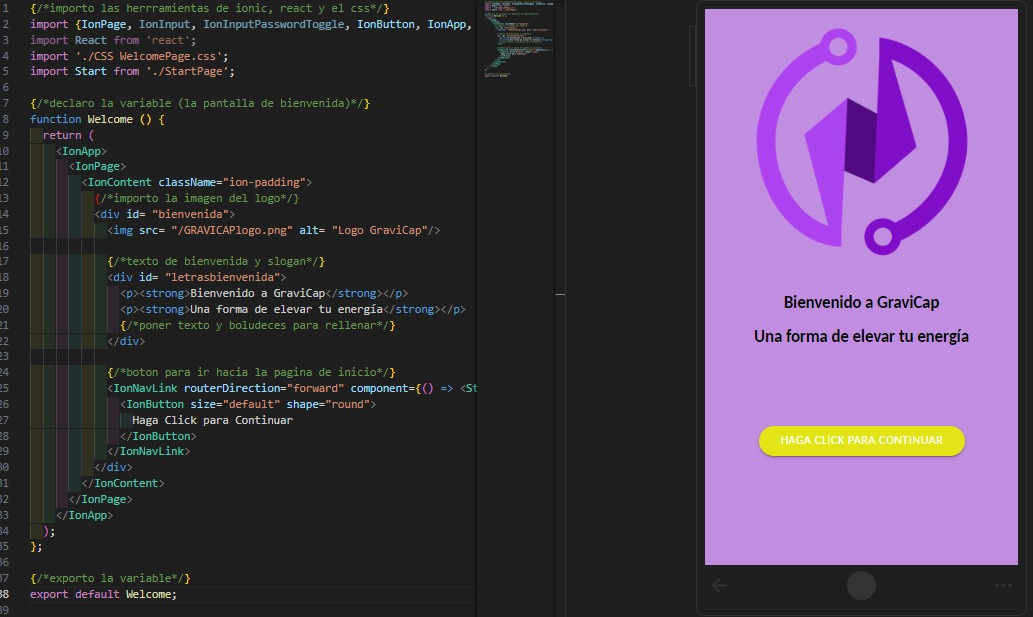
\includegraphics[width=\linewidth]{Imagenes/Aplicación/Code.jpg}
                        \caption{Imagen de Referencia de la función de Smartphone}
                        \label{fig:a15}
                    \end{figure}
        
                    Con los archivos desarrollados con sus componentes y estructuras, para el movimiento del usuario por las diferentes pantallas de estas, los componentes necesitan un enrutamiento para la conexión entre sí. Para esto, los componentes que provee Ionic como botones (\textit{ion-button}) o cartas (\textit{ion-card}) se los programó con la función de \textit{IonNavLink}, funciona como un enrutamiento, el cual realiza que al clickear un botón o carta nos redireccione hacia otro componente/archivo que le designemos. Con esto, el Usuario se puede movilizar dentro de la aplicación hacia donde necesite. Así también como se redirecciona hacia un componente, puede volver hacia atrás a la pantalla anterior, esto con la herramienta \textit{IonBackButton}.\par
                        
                    El usuario, en la pantalla de inicio, en la parte superior derecha de la misma, dispone de un botón de información, el cual, le proveerá información de nuestras redes sociales y contacto.\par
                    Para un mejor movimiento del usuario dentro de la aplicación, se implementó la herramienta \textit{Tabs} (\textit{ion-tabs}). Esta es una barra ubicada en la parte inferior la cual le permite al usuario moverse de una forma más eficiente, conteniendo iconos, los cuales actúan de botones para redireccionar al usuario hacia su determinada pantalla, dándole posibilidad de visualizar otras pantallas y obtener otro tipo de información.\par
                    Una vez teniendo todos los archivos programados con sus respectivas estructuras y componentes, se debe añadir estilos, darle forma a los componentes que queramos, colores y tamaños, dándoles así el vistazo estético requerido planteado en el Mockup. Para esto, cada componente necesita sus estilos, creándose así un archivo \textit{CSS} individual para cada uno. Estos se programan y se importan al archivo que se requiera, modificando su estructura y tamaños dándole un mejor acabado estético para el usuario.\par
                
            \subsection{Estilos y CSS}
                Una vez teniendo todos los archivos programados con sus respectivas estructuras y componentes, se debe añadir estilos, darle forma a los componentes que queramos, colores y tamaños, dándoles así el vistazo estético requerido planteado en el Mockup. Para esto, cada componente necesita sus estilos, creándose así un archivo CSS individual para cada uno. Estos se programan y se importan al archivo que se requiera, modificando su estructura y tamaños dándole un mejor acabado estético para el usuario.\par
                
            \subsection{Gráficos}
                Para el desarrollo de los gráficos dentro de la aplicación, se utilizaron las carpetas de \textbf{charts.js} y \textbf{react-chartjs-2}. De estas carpetas, importamos los tipos de gráficos que necesitemos para, posteriormente, programarlos y darles forma con los valores que registre la base de datos. Los tipos de gráficos que se utilizaron fueron: “\textit{Doughnut}” (circular); “\textit{Bar}” (columna) y “\textit{Line}” (línea).\par
                Para esto, se creó un archivo diferente para el desarrollo de cada gráfico para, posteriormente, importarlo hacia los archivos de los gráficos. Estos archivos, al ser JavaScript, los desarrollamos en formato .jsx.\par

                \subsubsection{Tipos de Gráficos Utilizados}
                \begin{itemize} [label=•]
                \setlength{\itemindent}{1.5em}
                
                    \item Doughnut\par
                        Este gráfico fue utilizado en el apartado de la Pantalla de Energía generada, dándonos un gráfico circular el cual se adapta al valor de energía que genere la batería.\par
                        
                    \item Bar\par
                        Para que el usuario pueda ver los valores cómodamente, además de tener una referencia de su magnitud, se usó este tipo de gráfico, el cual nos da los valores referenciados en columnas.\par
                        Estos valores son el Voltaje, Amperaje y Wataje (potencia) de la batería.\par
                        Este gráfico se utilizó en la Pantalla de Valores de la Batería.\par
                        
                    \item Line\par
                        Dentro de los gráficos de potencia podemos observar 2 gráficos del mismo tipo, siendo estos de línea. Para referencia el valor de potencia de la batería en función del tiempo se utilizó este tipo de gráfico.\par
                        Para la potencia de carga siendo un gráfico de línea ascendente y para la Potencia de descarga siendo un gráfico del mismo tipo pero descendente.\par
                \end{itemize}
                
            \subsection{Servidor}
                El microcontrolador utilizado para la creación del servidor, fue una ESP8266, comunicándose con la aplicación por medio de WiFi.\par
                Para el desarrollo de código se utilizó C++ con un sistema de detección del usuario al servidor conectado dentro de la misma red WiFi.\par
                Dentro del servidor se obtienen los valores y datos de los sensores de la etapa de control, dándonos así, valores de corriente; tensión; voltaje y carga de los 4 sensores utilizados.\par
                Cada sensor contiene información de datos diferentes, destinados a sensar específicamente una sección de la batería, como el panel solar, el consumo de la batería, el consumo de usuario y la potencia de la placa MPPT.\par
                Al ser 4 sensores con información de datos diferentes, para una petición más cómoda de datos, realizamos solicitudes individuales a cada uno de los sensores por separado.
                Cuando se realice una solicitud dentro del servidor y sea correcta y aceptada, este está configurado para contestar mandando los valores en formato de archivo json mandando un \textit{string} con los valores.\par
                Dentro del desarrollo de la aplicación, para pedir los datos de los sensores dentro de los archivos de las pantalla, realizamos un fetch el cual solicitará los datos en forma de GET a la IP del servidor al sensor específico que le indiquemos.\par
                Una vez realizado el fetch, obtendremos todos los valores del sensor al cual le indicamos la solicitud. Posteriormente, para mostrar los datos que necesitemos dentro de la pantalla de la aplicación, declaramos una variable la cual contendrá el dato específico que necesitemos del sensor recibido y la utilizamos dentro de la aplicación, mostrando el valor dentro del dispositivo móvil.\par

            \newpage
            
            \subsection{Android Studio}
                Una vez teniendo todo el desarrollo de código dentro de Visual Studio Code, realizamos el vistazo de la aplicación dentro de un dispositivo móvil android. Para lograr esto, utilizamos Android Studio el cual nos permitió realizar la conversión de nuestro proyecto de desarrollo en una aplicación móvil ejecutable dentro de nuestro dispositivo móvil android. Con esto, ya tenemos el vistazo final de la aplicación dentro de un dispositivo móvil, solamente pudiendo variar los tamaños de la aplicación debido a la resolución que tenga cada dispositivo donde se descargue.\par
                Con esto, se pudo modificar los tamaños para adaptarlo lo mejor posible teniendo de referencia un celular con la aplicación.\par
                Para una mejor estética, Android Studio nos permite modificar el nombre a la aplicación vista en el dispositivo móvil y también el logo que tendrá, dándonos así la posibilidad de modificarlo a nuestro gusto. Dando como resultado, el siguiente logotipo de aplicación para móviles.\par

                \begin{figure} [H]
                    \centering
                    
\includegraphics[width=0.5\linewidth]{Imagenes/Aplicación/Icon.jpg}
                    \caption{Icono de la aplicación que se ve al descargarla}
                    \label{fig:a21}
                \end{figure}
                
                Para que cualquier persona pueda descargar la aplicación en su dispositivo móvil, Android Studio también nos permite generar un archivo \textbf{\textit{.apk}}, el cual, es un archivo ejecutable que contiene la aplicación. Al abrir el archivo \textit{\textbf{apk}}, podrá instalar la aplicación en su dispositivo móvil.\par
\chapter{Estructura}
    \section{Materiales}
        \begin{itemize} [label=•]
        \setlength{\itemindent}{3em}
            \item 3 varas de 87 cm de largo y 8 milímetros de grosor.
            \item 1 vara en forma L de 82 cm de largo y 3 milímetros de grosor.
            \item 2 caños de 230 cm de largo y 7,5 cm de ancho. 
            \item 2 estructuras de caños de 98 cm de largo y 89 cm de alto. La superior tiene una polea y la estructura inferior tiene dos poleas.
            \item Placa MPPT.
            \item Placa del microcontrolador del MPPT.
            \item Placa step down.
            \item Placa etapa de control.
            \item Fuente de energía renovable (para este prototipo es un panel solar de 24 voltios).
            \item 6 metros de cable de acero sin recubrimiento de 6 milímetros de grosor.
            \item 1 peso de 30 kilogramos de cemento.
            \item 1 motor.
            \item 1 encoder.
        \end{itemize}
        
    \section{Herramientas}
        \begin{itemize} [label=•]
        \setlength{\itemindent}{3em}
            \item Llave Alem de 6mm.
            \item Llave de 17mm.
            \item Llave de 8mm.
            \item Soportes para el peso.
        \end{itemize}

    \section{Precauciones} 
        Al manipular o mover el peso de la batería se recomienda moverlo entre 2 personas para llevarlo más fácilmente, sugerimos la utilización de calzado de seguridad, guantes y un equipo adecuado para movilizarlo, como una carretilla o carro. Se debe manejar con cuidado para evitar la caída del peso, este puede causar lesiones en personas circundantes o los pisos.\par
        Asegurarse de que la energía generada por la batería sea adecuada para el dispositivo que requiera cargar, para evitar una posible sobrecarga en el dispositivo conectado, quemando o dañando los componentes que lo conforman.\par
        Verificar los valores de voltaje y/o corriente de forma periódica para estar al tanto de cambios repentinos o paulatinos en el funcionamiento del dispositivo.\par
        No realizar mantenimiento en la estructura mientras el cable esté colocado con el peso acoplado.
        Verificar que el cable de acero esté tensado de manera correcta y bien acoplado en el sistema de poleas.\par
        Al armar y desarmar la estructura se debe preveer un soporte para el peso, apoyándolo suavemente por medio de una descarga mientras le quita tensión al cable.\par
\chapter{Instalación}
    \section{Armado} 
        Este prototipo cuenta con un panel solar como medio de obtención de energía renovable, pero podría utilizarse cualquier otro tipo de generador de energía.\par
        Para evitar atenciones agravadas por la distancia recorrida a través de los cables de conexión, recomendamos colocar la batería cerca del panel solar, u otros, preferentemente en un ambiente cerrado o protegido de la intemperie.\par
        Luego de elegir un espacio protegido de la humedad u otros factores climáticos, alejado de zonas de tránsito recurrente, o habituadas por niños y animales, quitar el embalaje de todas las piezas y prepararlas para su posterior uso.\par
        Recomendamos observar continuamente la foto del dispositivo armado para chequear la posición de cada pieza.\par
        Al ajustar cada bulón, hace falta utilizar una llave de 17mm, y una llave álem de 6mm por el otro lado.\par
        Recomendamos contar con un juego de llaves criquet para facilitar el proceso. Ambas llaves colocadas en simultáneo, con la rosca preparada para un ajuste.\par
        Tener en cuenta, que luego de algunos armados y desarmados las roscas de los bulones y las tuercas pueden verse deterioradas, es importante observar particularmente este punto antes de cada instalación, y reemplazar las piezas en caso de ser necesario. Recomendamos reemplazar en su totalidad los 12 pares de bulón-tuerca cuando uno de ellos aparezca deteriorado.\par
        A continuación, los pasos a seguir:\par

        \begin{enumerate}
            \item Colocar la estructura inferior sobre el suelo.
            \item Tomar uno de los caños de 230cm, y posicionarlo en su lugar.
            \item Ajustar el bulón y la tuerca correspondiente a dicha unión.
            \item Tomar una vara de 87cm de largo, presentarla a modo de escuadra o soporte entre la estructura inferior y el caño vertical, colocado del lado externo a la estructura.
            \item Tomar el caño de 230cm restante y repetir los pasos 2, 3 y 4.
            \item Colocar los dos soportes o escuadras restantes, ajustando únicamente la parte inferior, la pieza quedará haciendo péndulo sobre el caño vertical.
            \item El paso que sigue es posicionar la estructura superior, para esto será necesaria la ayuda de otra persona, esta se quedará sosteniendo la estructura desde el frente, mientras la otra persona ajusta ambos lados de la pieza.
            \item Luego habrá que terminar de colocar los dos soportes colocados en el paso 6, la persona que se encuentra sosteniendo la estructura no podrá soltarla hasta que uno de los dos soportes esté ajustado totalmente.
        \end{enumerate}
        
        La estructura se encuentra armada, ahora hay que colocar el peso y la carga:\par

        \begin{enumerate}
            \item Presentar el motor del dispositivo sobre su respectivo soporte. Ajustar parcialmente la abrazadera a su alrededor.
            \item Tomar las dos varillas roscadas de 5 cm con sus respectivas tuercas y arandelas, ajustando ambas para que mantengan el motor en posición.
            \item Una vez ajustados los soportes, terminar de ajustar la abrazadera, el motor debe estar fijo en su posición.
            \item Tomar el encoder y asegurarlo a la polea adherida al motor. Dejar a disposición sus terminales para su posterior conexión.
            \item Colocar sobre el suelo, debajo de la estructura el banco de soporte previamente seleccionado para sostener el peso.
            \item Trasladar con ayuda de otra persona el mismo hasta posicionarlo sobre dicho banco. Es importante observar que el cable se encuentre adherido al peso por la parte inferior del mismo.
            \item Colocar el cable en los rieles de las 4 poleas.
            \item Asegurando que el ojo de gancho esté lo más abierto posible, colocar el acople 1 entre el peso y la punta del ojo de gancho que no está adherida al cable.
            \item Una vez colocado, cerrar el ojo de gancho lo máximo posible, asegurándose de no girar sobre sí mismo el cable. Recomendamos el uso de una varilla a modo de palanca.
        \end{enumerate}
        
        El dispositivo está armado, resta conectar el panel solar al sistema, el encoder y los terminales del motor.\par
        Asegurarse de que el panel solar se encuentre posicionado y con sus dos terminales disponibles para su conexión. Es importante que en ningún momento se toquen los terminales para evitar dañar el dispositivo.\par
        
        Finalmente:\par

        \begin{enumerate}
            \item Conectar los terminales del encoder a sus respectivas borneras, teniendo en cuenta:

            \begin{itemize} [label=-]
                \item Pin A: Verde
                \item Pin B: Blanco
                \item VCC: Rojo
                \item GND: Negro
                \item Malla de recubrimiento: Malla metálica
            \end{itemize}

            \begin{figure} [H]
                \centering
                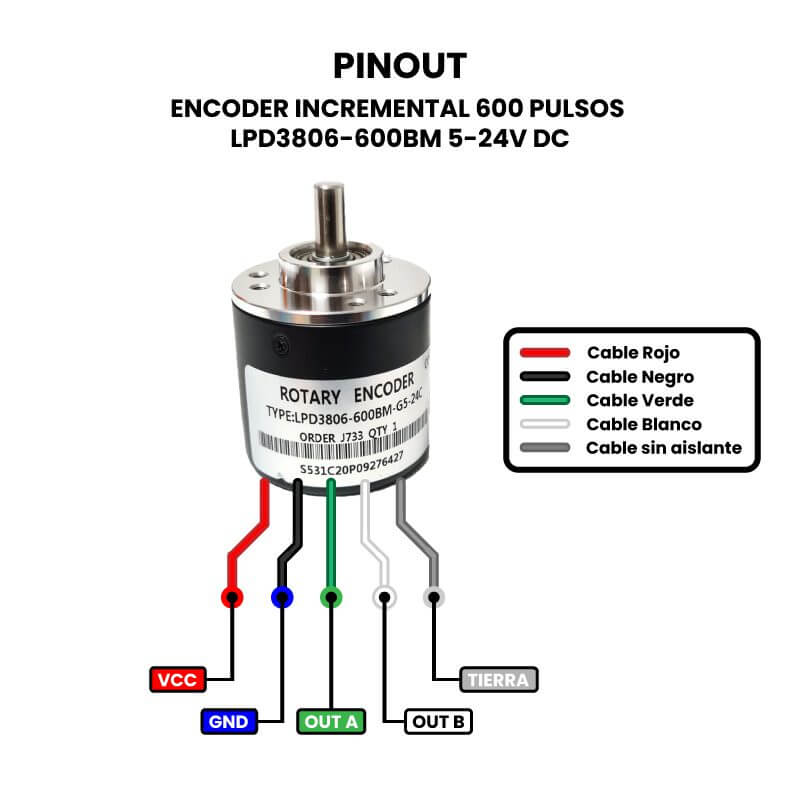
\includegraphics[width=0.5\linewidth]{Imagenes/Instalacion/Encoder.png}
            \end{figure}
            
            \item Conectar los terminales del motor a sus respectivas borneras.
            \item Conectar los terminales del panel solar a sus respectivas borneras.

        \end{enumerate}

        \begin{figure}
            \centering
            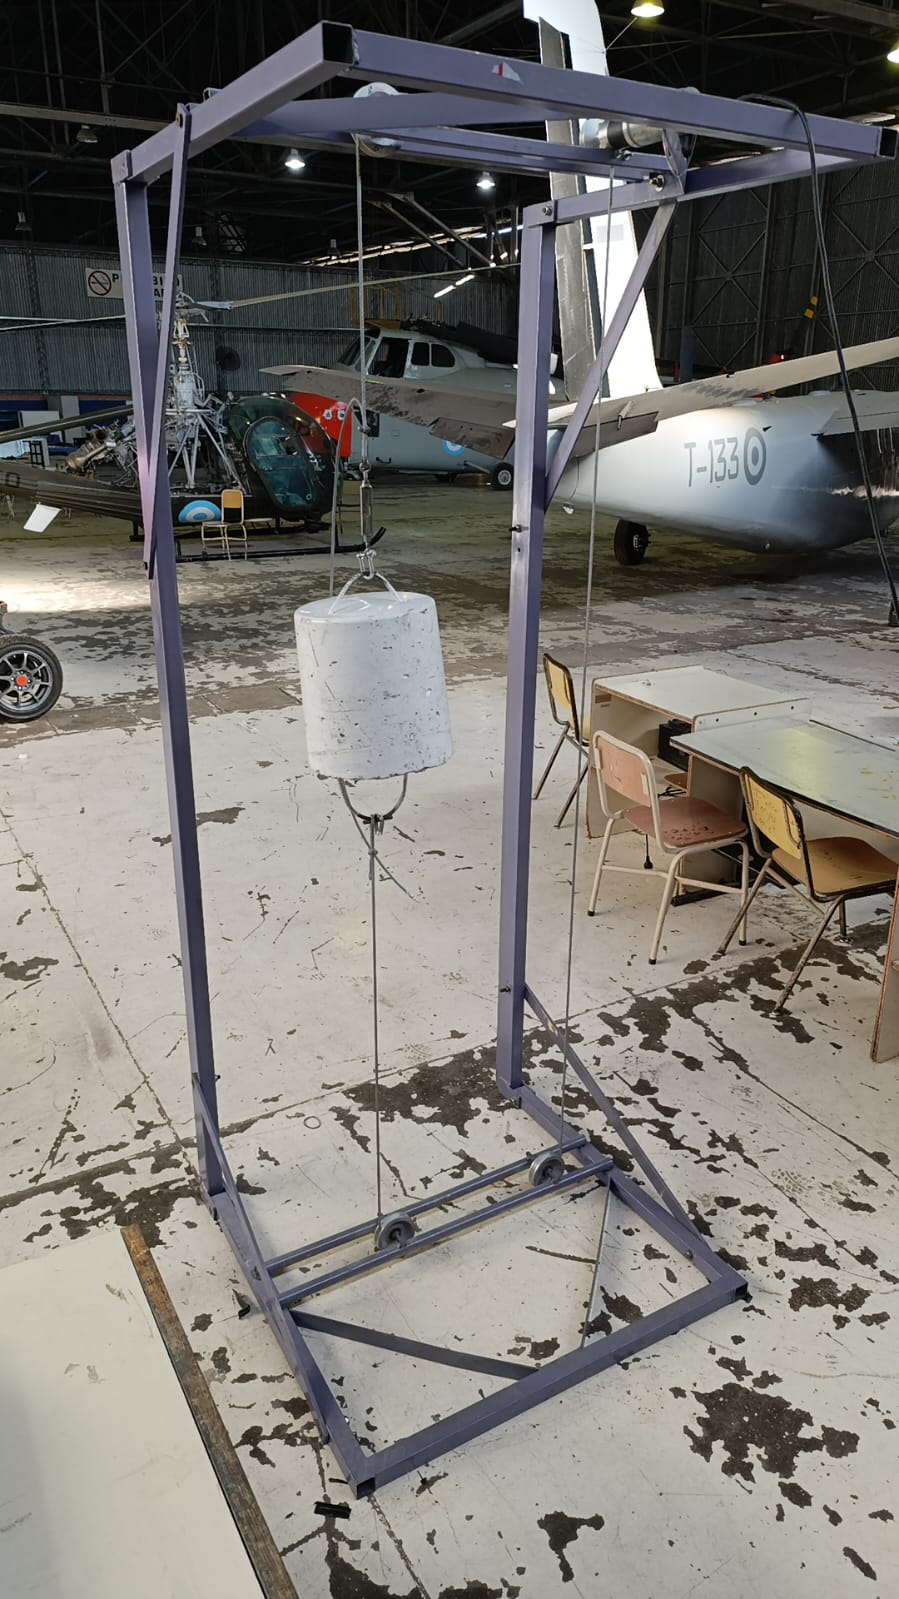
\includegraphics[width=0.5\linewidth]{Imagenes/Instalacion/Estructura.png}
        \end{figure}
\chapter{Contacto}

    \textbf{Link a la web:}
    \href{https://gravicap.vercel.app}{https://gravicap.vercel.app} 
    
    \textbf{Link a trello:}
    \href{https://trello.com/b/EtjuqFFQ/kanban}{https://trello.com/b/EtjuqFFQ/kanban}
    
    \textbf{Link a github:}
    \href{https://github.com/impatrq/gravicap}{https://github.com/impatrq/gravicap}
    
    \textbf{Link redes sociales:}
    \href{https://www.instagram.com/gravi.cap/}{https://www.instagram.com/gravi.cap/}

\end{document}